
\documentclass[handout]{beamer}\usepackage[]{graphicx}\usepackage[]{color}
%% maxwidth is the original width if it is less than linewidth
%% otherwise use linewidth (to make sure the graphics do not exceed the margin)
\makeatletter
\def\maxwidth{ %
  \ifdim\Gin@nat@width>\linewidth
    \linewidth
  \else
    \Gin@nat@width
  \fi
}
\makeatother

\definecolor{fgcolor}{rgb}{0.345, 0.345, 0.345}
\newcommand{\hlnum}[1]{\textcolor[rgb]{0.686,0.059,0.569}{#1}}%
\newcommand{\hlstr}[1]{\textcolor[rgb]{0.192,0.494,0.8}{#1}}%
\newcommand{\hlcom}[1]{\textcolor[rgb]{0.678,0.584,0.686}{\textit{#1}}}%
\newcommand{\hlopt}[1]{\textcolor[rgb]{0,0,0}{#1}}%
\newcommand{\hlstd}[1]{\textcolor[rgb]{0.345,0.345,0.345}{#1}}%
\newcommand{\hlkwa}[1]{\textcolor[rgb]{0.161,0.373,0.58}{\textbf{#1}}}%
\newcommand{\hlkwb}[1]{\textcolor[rgb]{0.69,0.353,0.396}{#1}}%
\newcommand{\hlkwc}[1]{\textcolor[rgb]{0.333,0.667,0.333}{#1}}%
\newcommand{\hlkwd}[1]{\textcolor[rgb]{0.737,0.353,0.396}{\textbf{#1}}}%
\let\hlipl\hlkwb

\usepackage{framed}
\makeatletter
\newenvironment{kframe}{%
 \def\at@end@of@kframe{}%
 \ifinner\ifhmode%
  \def\at@end@of@kframe{\end{minipage}}%
  \begin{minipage}{\columnwidth}%
 \fi\fi%
 \def\FrameCommand##1{\hskip\@totalleftmargin \hskip-\fboxsep
 \colorbox{shadecolor}{##1}\hskip-\fboxsep
     % There is no \\@totalrightmargin, so:
     \hskip-\linewidth \hskip-\@totalleftmargin \hskip\columnwidth}%
 \MakeFramed {\advance\hsize-\width
   \@totalleftmargin\z@ \linewidth\hsize
   \@setminipage}}%
 {\par\unskip\endMakeFramed%
 \at@end@of@kframe}
\makeatother

\definecolor{shadecolor}{rgb}{.97, .97, .97}
\definecolor{messagecolor}{rgb}{0, 0, 0}
\definecolor{warningcolor}{rgb}{1, 0, 1}
\definecolor{errorcolor}{rgb}{1, 0, 0}
\newenvironment{knitrout}{}{} % an empty environment to be redefined in TeX

\usepackage{alltt}
\usetheme[hideothersubsections,left]{Marburg}



\usepackage{pgfpages}
\usepackage{pgffor}
%\pgfpagesuselayout{4 on 1}[a4paper,landscape]

%\pagestyle{empty} % descomentar para impresión muy blanca

\usepackage[utf8]{inputenc}
\usepackage[catalan]{babel}
\usepackage{verbatim}
\usepackage{hyperref}
%\hypersetup{colorlinks=false,linkbordercolor=red,linkcolor=green,pdfborderstyle={/S/U/W 1}}
%\hypersetup{colorlinks=true,linkbordercolor=red,linkcolor=green,pdfborderstyle={/S/U/W 1}}
\hypersetup{colorlinks=true,linkcolor=blue,pdfborderstyle={/S/U/W 1}}

\usepackage{amsfonts,amssymb,amsmath,amsthm, wasysym}
\usepackage{listings}
\usepackage[T1]{fontenc}        
\usepackage{pgf}
\usepackage{epsdice}
\usepackage{pgfpages}
\usepackage{tikz}
\usetikzlibrary{arrows,shapes,plotmarks,backgrounds,trees,positioning}
\usetikzlibrary{decorations.pathmorphing,calc,snakes}
%\usepackage{marvosym}
%
%\usetheme[hideothersubsections,left]{Marburg}
%\usetheme[hideothersubsections,left]{Madrid}
%\usetheme[hideothersubsections,left]{Dresden}
%\usetheme{Darmstadt}
\usecolortheme{sidebartab}
\useinnertheme[shadow]{rounded}

% \useoutertheme[footline=empty,subsection=true,compress]{infolines}
% \useoutertheme[footline=empty,subsection=true,compress]{miniframes}
% \usefonttheme{serif}

\setbeamertemplate{caption}[numbered]
\setbeamertemplate{navigation symbols}{}


\newcommand{\red}[1]{\textcolor{red}{#1}}
\newcommand{\green}[1]{\textcolor{green}{#1}}
\newcommand{\blue}[1]{\textcolor{blue}{#1}}
\newcommand{\gray}[1]{\textcolor{gray}{#1}}
\renewcommand{\emph}[1]{{\color{red}#1}}

\setbeamertemplate{frametitle}
{\begin{centering}
\medskip
\color{blue}
\textbf{\insertframetitle}
\medskip
\end{centering}
}
\usecolortheme{rose}
\usecolortheme{dolphin}
\mode<presentation>


\newcommand{\CC}{\mathbb{C}}
\newcommand{\RR}{\mathbb{R}}
\newcommand{\ZZ}{\mathbb{Z}}
\newcommand{\NN}{\mathbb{N}}
\newcommand{\KK}{\mathbb{K}}
\newcommand{\MM}{\mathcal{M}}
%\newcommand{\dbinom}{\displaystyle\binom}

\newcommand{\limn}{{\displaystyle \lim_{n\to\infty}}}
\renewcommand{\leq}{\leqslant}
\renewcommand{\geq}{\geqslant}
\def\tendeix{{\displaystyle\mathop{\longrightarrow}_{\scriptscriptstyle
n\to\infty}}}

\newcommand{\matriu}[1]{\left(\begin{matrix} #1 \end{matrix}\right)}

% \newcommand{\qed}{\hbox{}\nobreak\hfill\vrule width 1.4mm height 1.4mm depth 0mm
%     \par \goodbreak \smallskip}
%
% %

\theoremstyle{plain}
\newtheorem{teorema}{Teorema}
%\newtheorem{prop}{Proposición}
\newtheorem{prop}{Propiedades}
\newtheorem{cor}{Corolario}
\theoremstyle{definition}
\newtheorem{Ejemplo}{Ejemplo}
\newtheorem{defin}{Definición}
\newtheorem{obs}{Observación}

\newcounter{seccions}
\newcommand{\seccio}[1]{\addtocounter{seccions}{1}
\medskip\par\noindent\textbf{\theseccions.
#1}\smallskip\par }

\newcommand{\EM}{\Omega}
\newcommand{\PP}{\mathcal{P}}

\title[\red{Matemáticas III GINF}]{}
\author[]{R. Alberich}
\date{}
\IfFileExists{upquote.sty}{\usepackage{upquote}}{}
\begin{document}
\beamertemplatedotitem

\lstset{backgroundcolor=\color{green!50}}
\lstset{breaklines=true}
\lstset{basicstyle=\ttfamily}


\section{Probabilidad}

\begin{frame}
\vfill
\begin{center}
\gray{\LARGE Probabilidades básicas}
\end{center}
\vfill
\end{frame}

\subsection{Definiciones básicas}

\begin{frame}
\frametitle{Definiciones básicas}

\emph{Experimento aleatorio:} experimento que  repetido  en las mismas condiciones puede  dar resultados diferentes, pero que a largo plazo son predecibles
\medskip

\blue{Ejemplo}: tirar  un dado  y contar los puntos de la cara superior
\bigskip

\emph{Suceso elemental:} cada uno de los posibles resultados del experimento aleatorio
\medskip

\blue{Ejemplo}: \epsdice{1}, \epsdice{2}, \epsdice{3}, \epsdice{4}, \epsdice{5}, \epsdice{6}
\bigskip


\emph{Espacio muestral:}  el conjunto  $\EM$ formado por todos los sucesos elementales del experimento aleatorio
\medskip

\blue{Ejemplo}: $\EM=\{\epsdice{1},\epsdice{2},\epsdice{3},\epsdice{4},\epsdice{5},\epsdice{6}\}$
\medskip

\end{frame}


\begin{frame}
\frametitle{Definiciones básicas}


\emph{Suceso:} cualquier subconjunto del espacio muestral.
\medskip

\blue{Ejemplo:} Alguno sucesos:
$$
\begin{array}{l}
\{\epsdice{1},\epsdice{2},\epsdice{3},\epsdice{4},\epsdice{5},\epsdice{6}\} \quad \mbox{(suceso \emph{seguro o cierto})}\\[1ex]
\emptyset\quad \mbox{(suceso \emph{imposible})}\\[1ex]
\{\epsdice{6}\}\\[1ex]
\{\epsdice{1},\epsdice{3},\epsdice{5}\}
\end{array}
$$


\red{$\PP(\EM)$:} conjunto de todos los sucesos del experimento aleatorio (conjunto de todos los subconjuntos de $\EM$)

\end{frame}


\begin{frame}
\frametitle{Ejemplo}

\emph{Experimento aleatorio:} escoger al  azar un 3-grama  (tres letras consecutivas contando los blancos de inicio y final de palabra) de la palabra "\_Baleares\_" 
\medskip

\emph{Espacio muestral:} $\EM=\{\_Ba, Bal, ale, lea, are, res, es\_\}$
\medskip

\emph{Algunos sucesos:}
$$
\begin{array}{l}
\{ale,are\} \quad \mbox{(3-gramas que empiezan por  $a$)} \\[2ex]
\{\_Ba,es\_\}\quad \mbox{(3-gramas de inicio y final de palabra)}\\[2ex]
\{Bal,ale,lea\} \quad \mbox{(3-gramas que contengan una ele)}
\end{array}
$$

\end{frame}


\subsection{Operaciones}
\begin{frame}
\frametitle{Operaciones con sucesos}

$A,B\subseteq \EM$:

\begin{itemize}
\item $\EM$: suceso \emph{total} o \emph{seguro}
\item $\emptyset$:suceso  \emph{vacío} o \emph{imposible}
\item $A\cup B$: suceso \emph{unión}; el que ocurre si sucede $A$ o $B$
\item $A\cap B$: suceso \emph{intersección}; el que ocurre si sucede $A$ y $B$
\item $A^c$: suceso \emph{complementario}  el que sucede si NO sucede $A$.
\item $A- B=A\cap B^c$: suceso \emph{diferencia} (el que acontece  si sucede $A$ y NO sucede $B$.
\end{itemize}

$A$ y $B$ son \emph{incompatibles} (o \emph{disjuntos}) cuando  $A\cap B=\emptyset$

\end{frame}

\begin{frame}
\frametitle{Ejemplo}

Supongamos que el sexo se divide entre Mujeres y Hombres.

$\blue{\EM=}\{\mbox{Estudiantes de esta clase}\}$\\
$\blue{A=}\{\mbox{Mujeres de esta clase}\}$\\
$\blue{B=}\{\mbox{Estudiantes que son zurdos}\}$\\
\begin{itemize}
\item $\blue{A\cup B=}\{\mbox{Est. que son mujeres o que son zurdos}\}$\medskip

\item $\blue{A\cap B=}\{\mbox{Mujeres de esta clase que son zurdas}\}$\medskip

\item $\blue{A^c=}\{\mbox{Hombres de esta clase}\}$\medskip

\item $\blue{A-B=}\{\mbox{Mujeres de la clases que \emph{no} son zurdas}\}$\medskip

\item $\blue{B-A=}\{\mbox{Hombres de la clase que son zurdos}\}$\medskip
\pause

\item No son incompatibles {\large\red{\smiley}}
\end{itemize}

\end{frame}


\begin{frame}
\frametitle{Propiedades}
\begin{enumerate}
\only<1>{\item[(a)] \emph{Conmutativas:} $A\cup B=B\cup A$, $A\cap B=B\cap A$\medskip

\item[(b)] \emph{Asociativas:} $A\cup(B\cup C)=(A\cup B)\cup C$, $A\cap(B\cap C)=(A\cap B)\cap C$}

\only<2>{\item[(c)] \emph{Distributivas:} $A\cap(B\cup C)=(A\cap B)\cup (A\cap C)$, $A\cup(B\cap C)=(A\cup B)\cap (A\cup C)$
%\medskip
}
\end{enumerate}

\end{frame}


\begin{frame}
\frametitle{Propiedades: gráficos}

\begin{center}
\begin{tabular}{ccc}
\hspace*{-1.5cm}  $A$ & $B\cap C$ & $A\cup (B\cap C)$\\
\hspace*{-1.5cm} 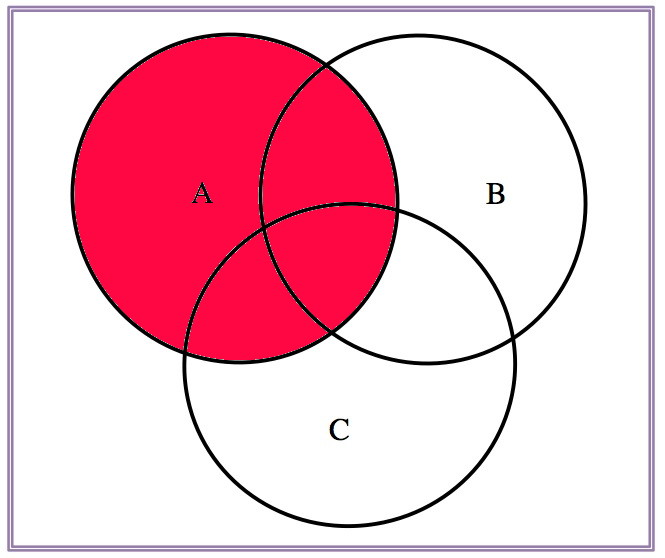
\includegraphics[width=0.25\linewidth]{distr11.jpg} &
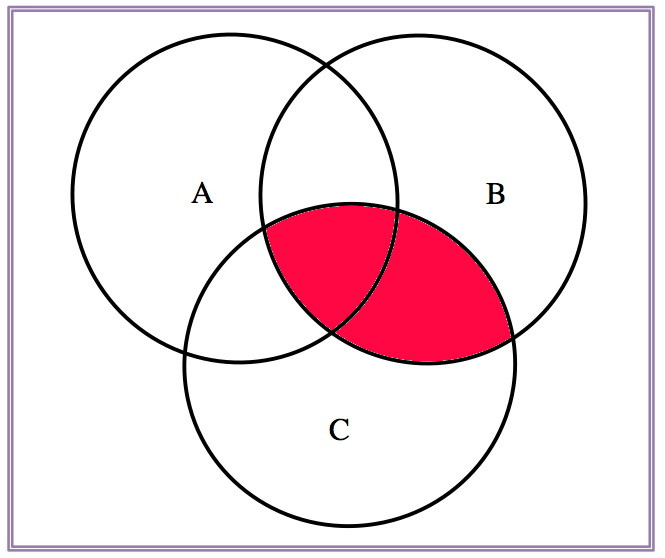
\includegraphics[width=0.25\linewidth]{distr12.jpg} &
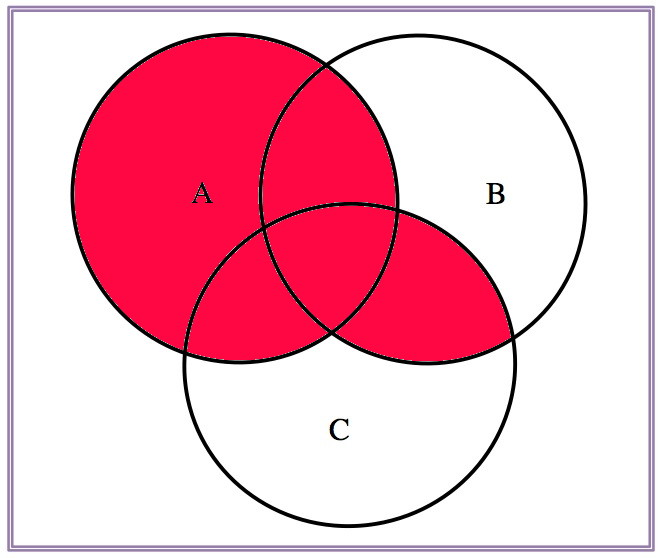
\includegraphics[width=0.25\linewidth]{distr13.jpg}\\[2ex]
\hspace*{-1.5cm} $A\cup B$ & $A\cup C$ & $(A\cup B)\cap (A\cup C)$\\
\hspace*{-1.5cm}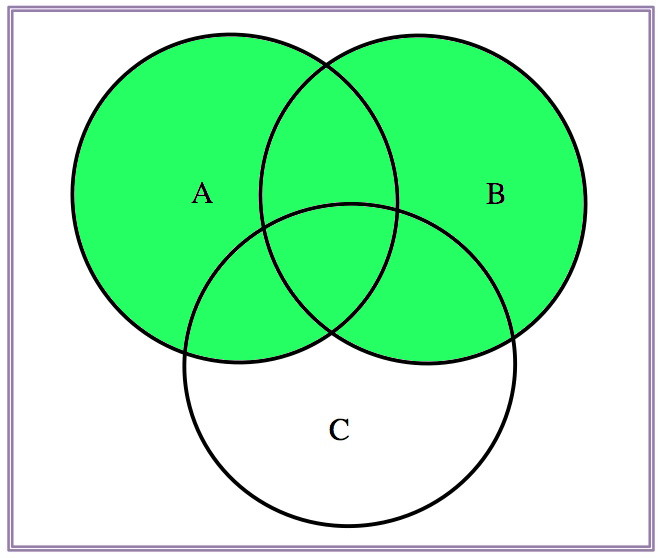
\includegraphics[width=0.3\linewidth]{distr21.jpg} &
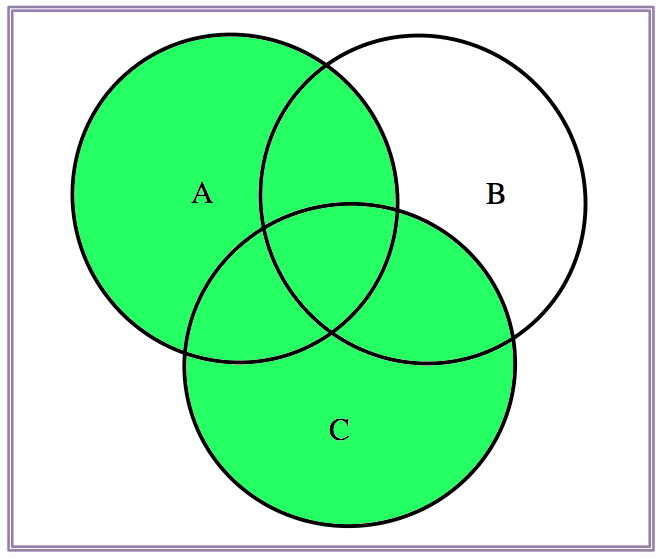
\includegraphics[width=0.25\linewidth]{distr22.jpg} &
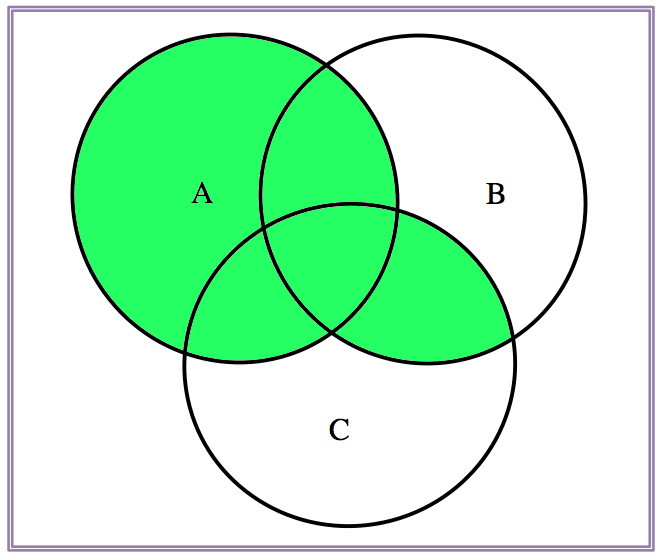
\includegraphics[width=0.25\linewidth]{distr23.jpg}\\ 
\end{tabular}
\end{center}
\end{frame}


\begin{frame}

\begin{enumerate}
%\only<3>{
\item[(d)] \emph{complementario del complementario:} $(A^c)^c=A$
\medskip
\begin{center}
\begin{tabular}{ccc}
\hspace*{-1cm}  $A$ & $A^c$ & $(A^c)^c$\\
\hspace*{-1cm} 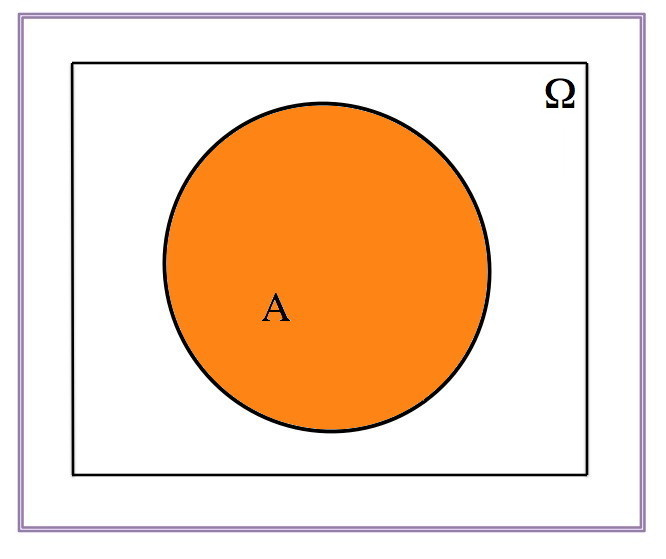
\includegraphics[width=0.3\linewidth]{dd2.jpg} &
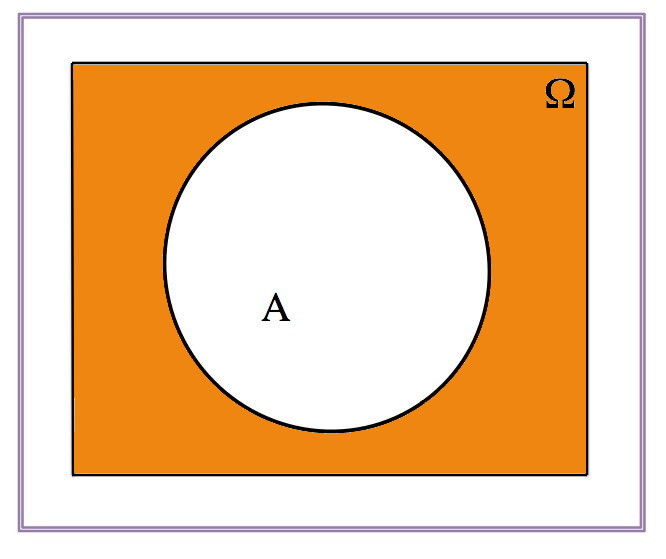
\includegraphics[width=0.3\linewidth]{dd1.jpg} &
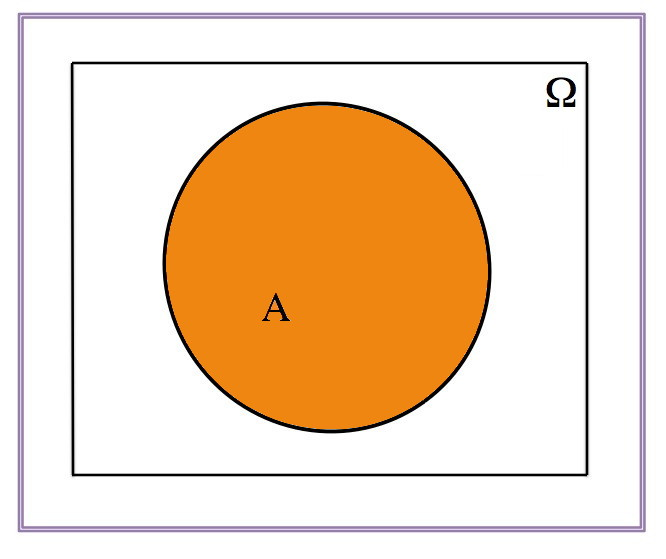
\includegraphics[width=0.3\linewidth]{dd3.jpg}
\end{tabular}
\end{center}
%}
\end{enumerate}

\end{frame}


\begin{frame}
\begin{enumerate}
%\item[(EEEE)] AAAAAAAAAAAAAAAAAAAAAAAAAAAAAAAAAAAAAAAAAAAAAAAAAAAAAAAAAAAAAAAAAA
%\only<4>{
\item[(e)] \emph{Leyes de De Morgan:} $(A\cup B)^c=A^c\cap B^c$, $(A\cap B)^c=A^c\cup B^c$
\medskip
\begin{center}
\begin{tabular}{cc}
\hspace*{-1cm}  $A\cup B$ & $(A\cup B)^c$ \\
\hspace*{-1cm} 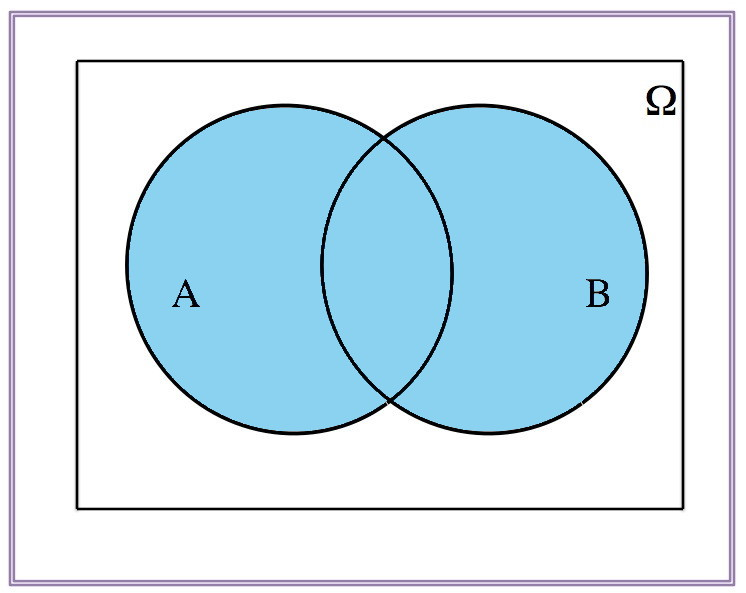
\includegraphics[width=0.3\linewidth]{demorgan6.jpg} &
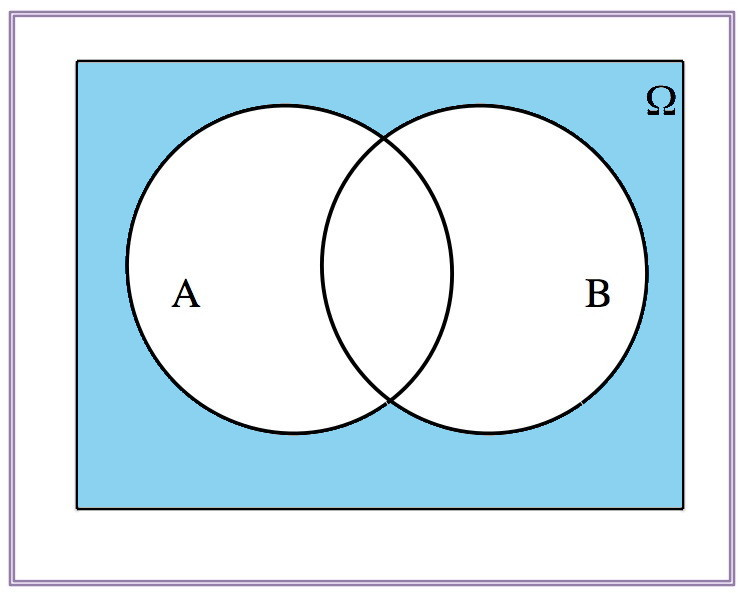
\includegraphics[width=0.3\linewidth]{demorgan7.jpg} \end{tabular}\\[2ex]
\begin{tabular}{ccc}
\hspace*{-1cm}  $A^c$ & $B^c$ & $A^c\cap B^c$\\
\hspace*{-1cm} 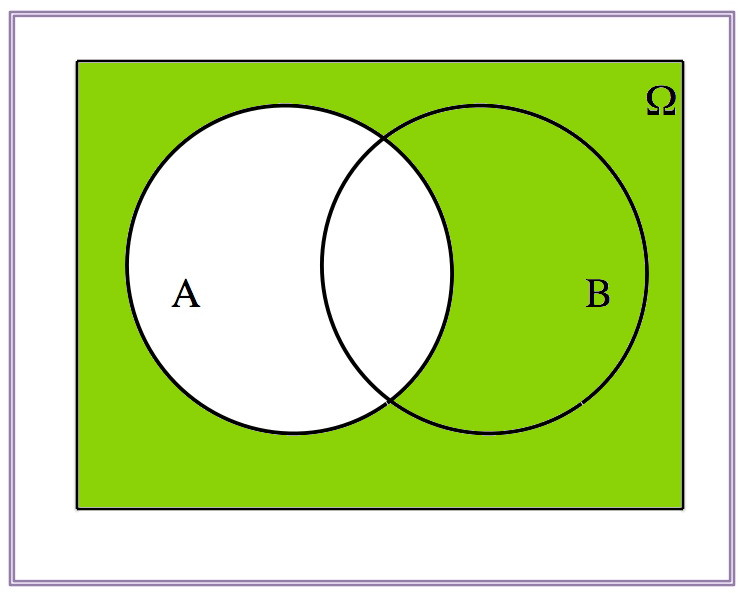
\includegraphics[width=0.3\linewidth]{demorgan8.jpg} &
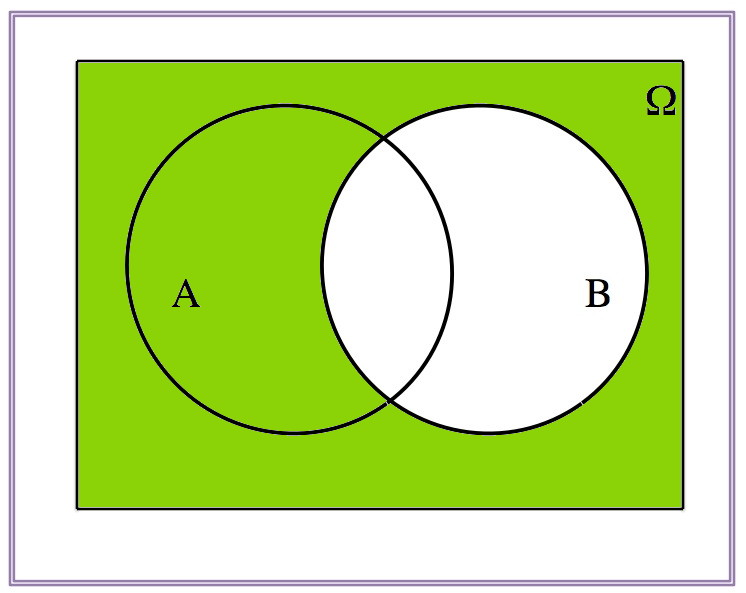
\includegraphics[width=0.3\linewidth]{demorgan9.jpg} & 
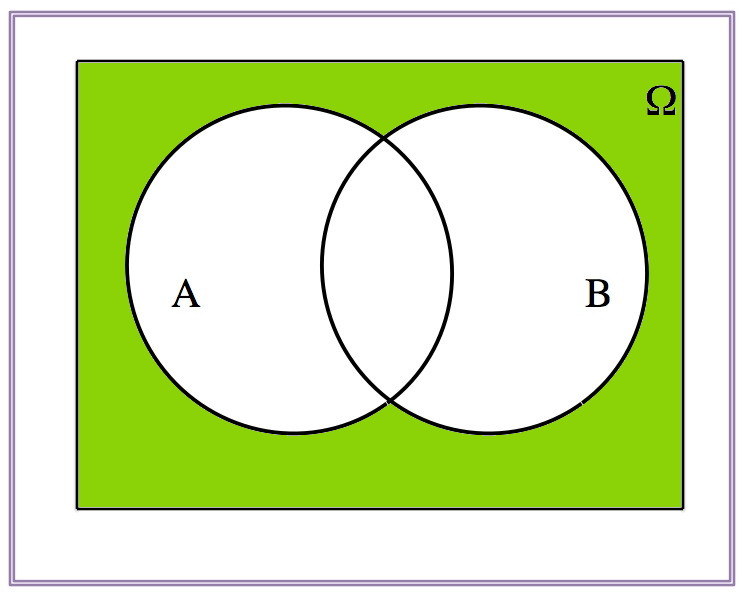
\includegraphics[width=0.3\linewidth]{demorgan10.jpg}
\end{tabular}\\[2ex]

\end{center}
%}
\end{enumerate}
\end{frame}

\begin{frame}

\begin{enumerate}
%5\only<5>{
\item[(e)] \emph{Leyes de De Morgan:} $(A\cup B)^c=A^c\cap B^c$, $(A\cap B)^c=A^c\cup B^c$
\medskip

\begin{center}
\begin{tabular}{cc}
\hspace*{-1cm}  $A\cap B$ & $(A\cap B)^c$ \\
\hspace*{-1cm} 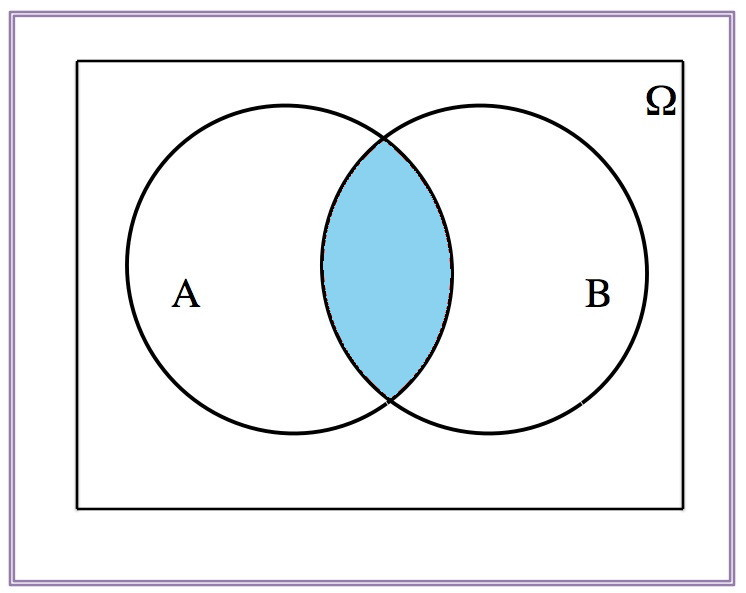
\includegraphics[width=0.3\linewidth]{demorgan1.jpg} &
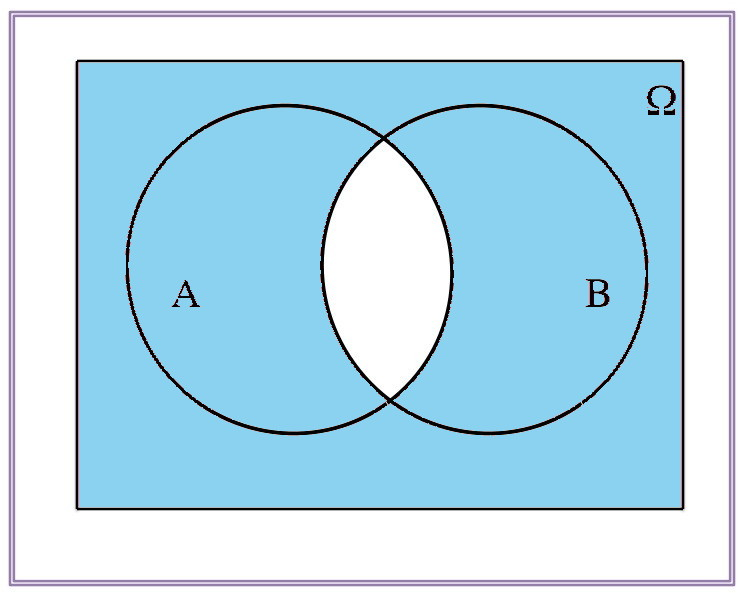
\includegraphics[width=0.3\linewidth]{demorgan2.jpg} \end{tabular}\\[2ex]
\begin{tabular}{ccc}
\hspace*{-1cm}  $A^c$ & $B^c$ & $A^c\cup B^c$\\
\hspace*{-1cm} 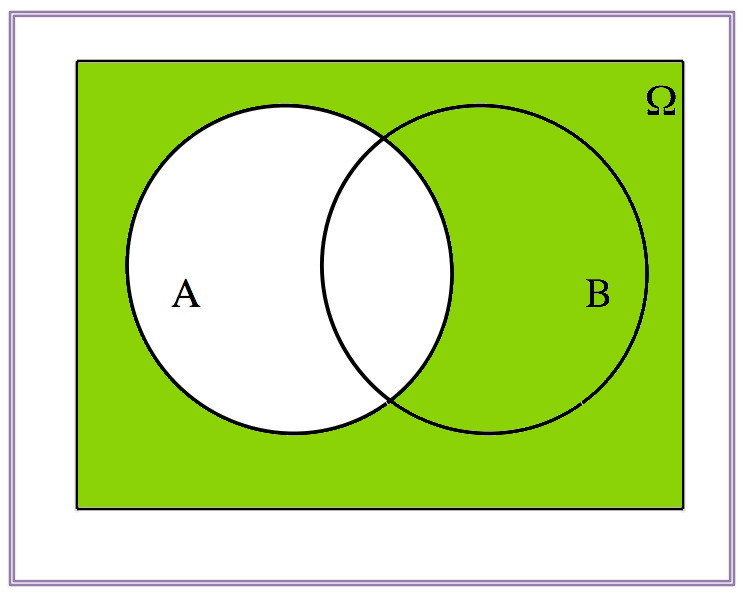
\includegraphics[width=0.3\linewidth]{demorgan3.jpg} &
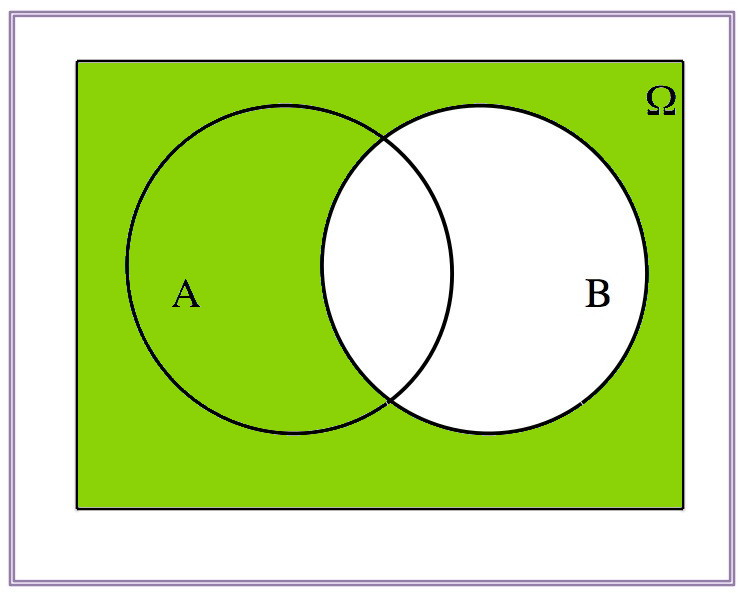
\includegraphics[width=0.3\linewidth]{demorgan5.jpg} & 
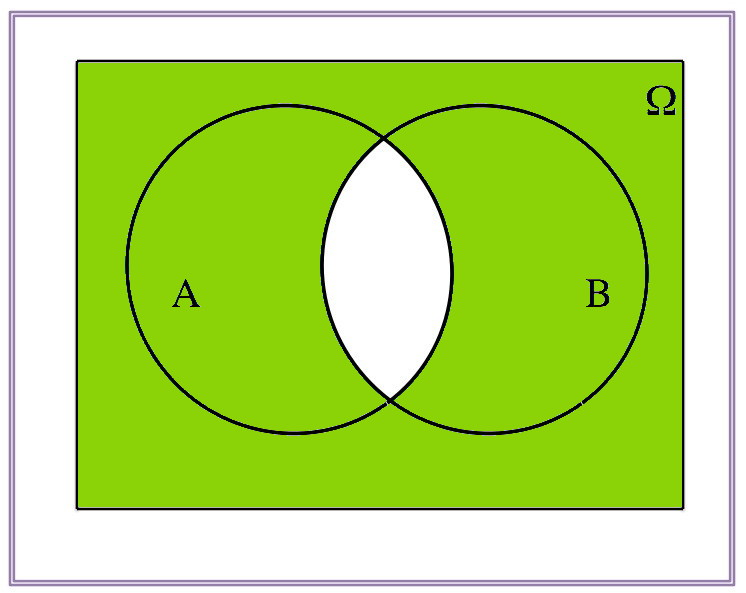
\includegraphics[width=0.3\linewidth]{demorgan4.jpg}
\end{tabular}\\[2ex]

\end{center}
%}
\end{enumerate}

\end{frame}



\subsection{Probabilidad}
\begin{frame}
\frametitle{Definición de probabilidad}

La probabilidad de un suceso es una puntuación (\textsl{score}) numérico entre 0 y 1 que mide la verosimilitud de que este evento se produzca.
\medskip

Esta verosimilitud puede estar justificada por 
\begin{itemize}
\item Estimación personal
\item Estimación de expertos
\item La frecuencia con la que se da 
\item Cálculo formal
\end{itemize}

\end{frame}


\begin{frame}
\frametitle{Definición de probabilidad}
\vspace*{-1ex}

Sea $\EM$ el espacio muestral de un experimento aleatorio. 
\emph{Supongamos que el número de posibles resultados, por el momento, es finito.}

Una \emph{probabilidad} sobre $\EM$ es una aplicación
$$
P:{\cal P}(\EM)\to [0,1]
$$
con las siguientes propiedades:

\begin{enumerate}[a)]
\item $0\leq P(A)\leq 1$, para todo suceso $A$ 
\item $P(\EM)=1$
\item Si $\{A_1,A_2,\ldots,A_n\}$ son sucesos disjuntos dos a dos, entonces

$$
P(A_1\cup A_2\cup \cdots \cup A_n)=P(A_1)+P(A_2)+\cdots +P(A_n)
$$
\end{enumerate}

Si $a\in \Omega$ es un suceso elemental cometeremos el abuso de notación de poner $P(a)$ en lugar de $P(\{a\})$
\end{frame}

\begin{frame}
\frametitle{Ejemplo}
\vspace*{-1ex}


En la página de la \href{http://www.donasang.org/que-es-la-sang/es_frequencies-dels-diferents-grups.html}{\blue{Fundación Banco de Sangre y Tejidos de las Islas Baleares}} podemos encontrar información sobre los porcentajes de tipos de sangre de los donantes de las Islas Baleares: 

\begin{center}
A: 46\%;\ B: 7.5\%; AB: 3.5\%; O: 43\%
\end{center}
¿Cuál es la probabilidad de que un balear donante de sangre  no  sea del  tipo 0?
\medskip

\red{Experimento aleatorio:} tipo de sangre  de un paciente humano
\medskip

\red{$\Omega=$}$\{\mbox{A,B,AB,O}\}$
\medskip

\red{Probabilidad} de un suceso: se asimila al porcentaje observado de individuos
\medskip

\red{Suceso:} $\{\mbox{O}\}^c=\{\mbox{A,B,AB}\}$
\bigskip

$\red{P(\{\mbox{O}\}^c)}\!=\!P(\{\mbox{A,B,AB}\})\!=\!
P(\mbox{A})+P (\mbox{B})+P(\mbox{AB})\!=\!0.55$
\end{frame}

\begin{frame}
\frametitle{Propiedades}
\vspace*{-2ex}

\begin{enumerate}[(a)]
\only<1>{\item[(a)] $P(\emptyset)=0$
\medskip

\item[(b)] $P(A-B)=P(A)-P(A\cap B)$\\
porque $P(A)=P(A-B)+P(A\cap B)$
\medskip

\begin{center}
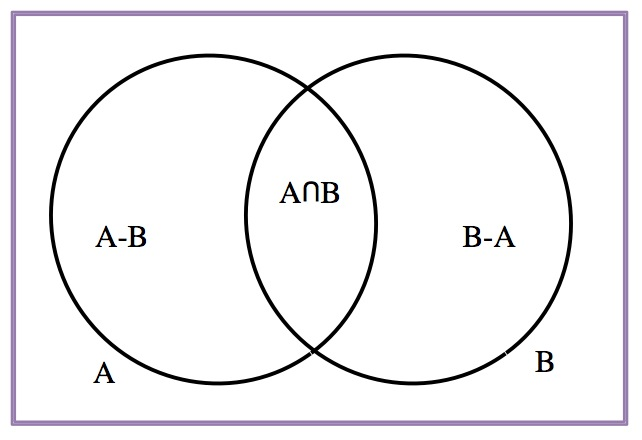
\includegraphics[width=0.6\linewidth]{A-B.jpg}
\end{center}


\item[(c)] Si $B\subseteq A$, entonces $0\leq P(B)\leq P(A)$
\medskip

\item[(d)] $P(A^c)=1-P(A)$
\medskip
}
\end{enumerate}
\end{frame}

\begin{frame}
\frametitle{Propiedades}
\begin{enumerate}[(a)]
\only<1>{\item[(e)] $P(A\cup B)=P(A)+P(B)-P(A\cap B)$ porque
{
\hspace*{-1.3cm}
\begin{eqnarray*}
& P(A)+P(B)-P(A\cap B)= P(A-B)+P(A\cap B)\\
& + P(B-A)+ P(A\cap  B)-P(A\cap  B)\\
& =P(A-B)+P(A\cap B)+ P(B-A)=P(A\cup B)
\end{eqnarray*}

}\medskip

\begin{center}
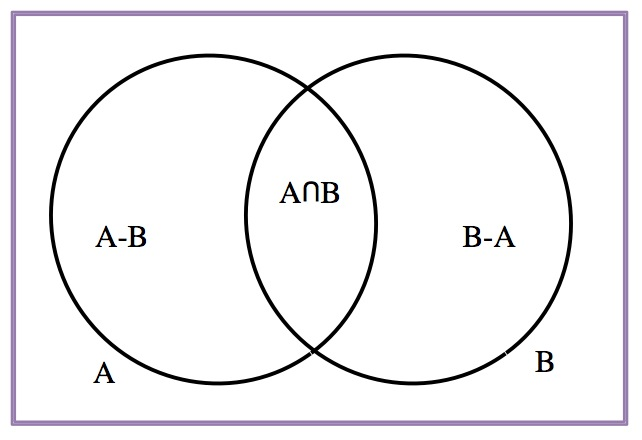
\includegraphics[width=0.6\linewidth]{A-B.jpg}
\end{center}
}
\end{enumerate}
\end{frame}

\begin{frame}
\frametitle{Propiedades}
\begin{enumerate}[(a)]
\only<1>{\item[(f)] $P(A\cup B\cup C)=P(A)+P(B)+P(C)$\\ \qquad $-P(A\cap B)-P(A\cap C)-P(B\cap C)$\\ \qquad $+P(A\cap B\cap C)$
\medskip

\begin{center}
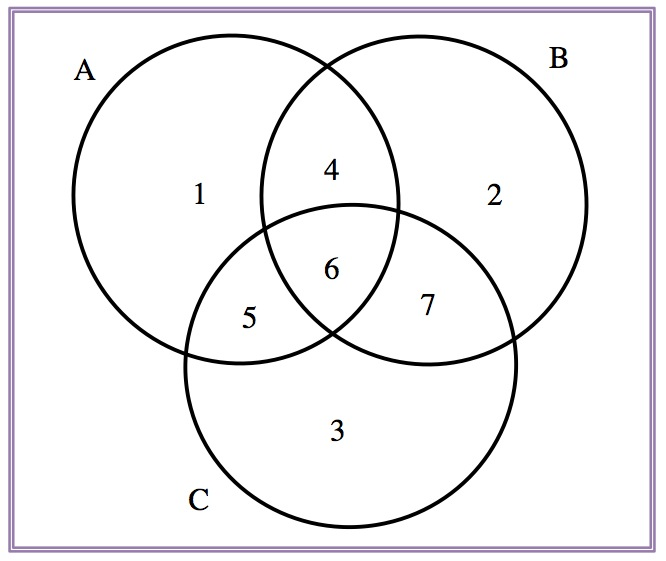
\includegraphics[width=0.7\linewidth]{tresconjunts.jpg}
\end{center}
\footnotesize{
$P(A\cup B\cup C)=P(1)+P(2)+P(3)+P(4)+P(5)+P(6)+P(7)$
}
}
\end{enumerate}
\end{frame}
%\end{document}
\begin{frame}
\frametitle{Propiedades}
\begin{enumerate}[(a)]
\item[(g)] Si $A=\{a_1,a_2,\ldots,a_k\}$, entonces
$$
P(A)=P(a_1)+P(a_2)+\cdots+P(a_k)
$$

\item[(h)] Si todos los sucesos elementales tienen la misma probabilidad,
$$
P(A)=\frac{|A|}{|\Omega|}\Big(=\frac{\mbox{casos favorables}}{\mbox{casos posibles}}\Big)
$$
\end{enumerate}
\end{frame}


\begin{frame}
\frametitle{Ejemplos}

Los porcentajes de vocales de un determinado idioma (de alfabeto latino) son:
%%%%%%https://es.wikipedia.org/wiki/Frecuencia_de_aparici%C3%B3n_de_letras

\begin{center}
A: 18.7\%; E: 26.1\%; I: 25.7\%; O: 24.4\% U: 5.1\%
\end{center}

¿Cuál es la probabilidad que vocal escogida al azar de este idioma sea una E o una O?
\medskip

$\Omega=\{A,E,I,O,U\}$
\medskip

Suceso$=\{E,0\}$
\bigskip

$P(\{E,I\})=P(E)+P(O)=0.261+0.244=0.505$


\end{frame}

\begin{frame}
\frametitle{Ejemplo}

%https://elpais.com/politica/2019/01/02/actualidad/1546426491_623324.html
%cocaína, metanfetamina, opiáceos, cannabis y anfetaminas

En un control especial de la policía el $0.1\%$ de todos los conductores analizados en un control de tráfico dan  positivo en un el test  en cocaína, y  el $1\%$ da positivo  en cannabis. Un $1.05\%$ da positivo en alguno de los dos test. \medskip

\blue{¿Cuál  es la probabilidad que un individuo analizado  en el control de drogas  escogido  al azar no de positivo  en ninguno de lo dos test?}
\medskip

$A$: dar positivo  en cocaína; $P(A)=0.001$
\medskip

$B$: dar positivo en cannabis; $P(B)=0.01$
\medskip

$A\cup B$: dar positivo en alguno de los dos test; $P(A\cup B)=0.0105$
\medskip

$(A\cup B)^c$: no dar positivo en ninguno de los test
\bigskip

$P((A\cup B)^c)=1-P(A\cup B)=1-0.0105=0.9895$
\end{frame}



\begin{frame}
\frametitle{Ejemplos}

En un control especial de la policía el $0.1\%$ de todos los conductores analizados en un control de tráfico dan  positivo en un el test  en cocaína, y  el $1\%$ da positivo  en cannabis. Un $1.05\%$ da positivo en alguno de los dos test. \medskip


\blue{¿Cuál  es la probabilidad que un analizado  al azar de positivo en los dos test en cocaína y cannabis?}
\medskip

$A$: dar positivo en cocaína; $P(A)=0.001$
\medskip

$B$: dar positivo en cannabis; $P(B)=0.01$
\medskip

$A\cup B$: dar positivo en algún de los dos test; $P(A\cup B)=0.0105$
\pause\medskip

$A\cap B$: dar positivo en los dos test
\bigskip

$\begin{array}{rl}
{P(A\cap B)} &{=P(A)+P(B)-P(A\cup B)}\\ &{=0.001+0.01-0.0105=0.0005}
\end{array}$
\end{frame}


\begin{frame}
\frametitle{Ejemplos}


En un control especial de la policía el $0.1\%$ de todos los conductores analizados en un control de tráfico dan  positivo en un el test  en cocaína, y  el $1\%$ da positivo  en cannabis. Un $1.05\%$ da positivo en alguno de los dos test. \medskip


\blue{¿Cuál es la probabilidad de  que un conductor analizado de  positivo en cocaína pero no en cannabis?}
\pause\medskip

$A$: dar positivo en cocaína; $P(A)=0.001$
\medskip

$B$: dar positivo en cannabis; $P(B)=0.01$
\medskip

$A\cap B$: dar positivo en los dos test; $P(A\cap B)=0.0005$
\medskip


$B-A$: dar positivo en  cocaína pero no en cannabis
\bigskip

$P(B-A) =P(B)-P(A\cap B) =0.01-0.0005=0.0095$
\end{frame}



\subsection{Probabilidad condicionada}
\begin{frame}
\frametitle{Probabilidad condicionada}

Dados dos sucesos  $A$  y $B$, con $P(A)>0$, la  \emph{probabilidad $P(B|A)$ de $B$ condicionado a $A$} es la probabilidad
\begin{itemize}
\item de que suceda  $B$ suponiendo que pasa $A$ 
\item de que si pasa $A$, entonces suceda $B$
\item de que un resultado de $A$ también pertenezca a $B$
\end{itemize}
\medskip

Se calcula así:

$$
P(B|A)=\frac{P(A\cap B)}{P(A)}
$$


\end{frame}

\begin{frame}
\frametitle{Ejemplo}

En una clase de 20 hombres  y 30 mujeres, 15 hombres y 18 mujeres llevan gafas.
\medskip

\begin{enumerate} 
\item[(1)] ¿Cuál es la probabilidad de que un alumno lleve gafas?
\pause$$
\frac{33}{50}
$$
\pause
\item[(2)] ¿Cuál es la probabilidad de que un alumno sea mujer y lleve gafas?
\pause$$
\frac{18}{50}
$$
\end{enumerate}

\end{frame}

\begin{frame}
\frametitle{Ejemplo}

En una clase de 20 hombres  y 30 mujeres, 15 hombres y 18 mujeres llevan gafas.
\medskip


\begin{enumerate} 

\item[(3)]  ¿Cuál es la probabilidad de que un chica lleve gafas?
\pause
$$
\frac{18}{30}=\frac{18/50}{30/50}\pause=\frac{P(\mbox{mujer  y gafas})}{P(\mbox{mujer})}
$$
\pause

\item[(4)] Si escogemos un estudiante al azar ¿Cuál es la probabilidad que si es mujer, entonces lleve gafas?
\pause
$$
\frac{18}{30}
$$
\end{enumerate}

\end{frame}




\begin{frame}
\frametitle{Ejemplo}

En una clase de 20 hombres  y 30 mujeres, 15 hombres y 18 mujeres llevan gafas.
\medskip


\begin{enumerate} 
\item[(5)]  ¿Cuál es la probabilidad de que un alumno que lleve gafas sea mujer?
\pause
$$
\frac{18}{33}=\frac{18/50}{33/50}=\frac{P(\mbox{mujer y gafas})}{P(\mbox{gafas})}
$$
\pause

\item[(6)] Si escogemos un estudiante al azar  ¿Cuál es la probabilidad de que si lleva gafas, entonces sea mujer?
$$
\frac{18}{33}
$$
\end{enumerate}

\end{frame}


\begin{frame}
\frametitle{Alerta}

Hay que distinguir bien entre
\begin{itemize}
\item $P(A\cap B)$: probabilidad de $A$ \red{y} $B$

\begin{quote}
Probabilidad de que sea mujer y  lleve gafas
\end{quote}
\medskip


\item $P(A|B)$: probabilidad de que \red{si} pasa $B$, \red{entonces} pase $A$

\begin{quote}
Probabilidad de que, si es mujer, lleve gafas
\end{quote}

\end{itemize}
\bigskip

Cuando utilizamos probabilidad condicional  $P(A|B)$ estamos restringiendo el espacio muestral a $B$
\end{frame}
\begin{frame}
\frametitle{Probabilidad condicionada. Propiedades}

La probabilidad condicionada es una probabilidad

\begin{prop}
Sea $A\subseteq \EM$ un suceso tal que $P(A)>0$. entonces
$$
\begin{array}{rccl}
P(-|A):& \mathcal{P}(\EM) & \to & [0,1]\\
&B & \mapsto & P(B|A)
\end{array}
$$
satisface las propiedades de las probabilidades
\end{prop}

Por ejemplo:
$$
\begin{array}{l}
P(B^c|A)=1-P(B|A)\\
P(B_1\cup B_2|A)=P(B_1|A)+P(B_2|A)-P(B_1\cap B_2|A)
\end{array}
$$

\end{frame}

%\begin{frame}
%\frametitle{Ejemplos}
%
%Una espècie de pèsols pot produir flors blanques o vermelles. Aquesta propietat depèn d'un sol gen amb dos a\l.lels, $C$ (vermell) i $c$ (blanc). Cada planta té dos gens que determinen el color de la flor, cada un provenint d'una planta progenitora. $C$ és dominant.
%
%Si creuam dues plantes de tipus $Cc$, quina és la probabilidad que la planta filla sigui  $CC$ sabent que té les flors vermelles?
%\medskip
%
%$A$: tenir les flors vermelles; $P(A)=0.75$
%\medskip
%
%$B$: ser $CC$; $P(A\cap B)=P(B)=0.25$
%\bigskip
%
%{$\displaystyle P(B|A)=\frac{P(B\cap A)}{P(A)}=\frac{0.25}{0.75}=\frac{1}{3}$}
%\end{frame}

\begin{frame}
\frametitle{Ejemplos}

Un 15\% de los adultos son hipertensos, un 25\% de los adultos creen que son hipertensos, y un 9\% de los adultos son hipertensos y creen que lo son.
\medskip

\blue{Si un adulto cree que es hipertenso, cuál es la probabilidad que lo sea?}
\medskip

$A$: ser hipertenso; $P(A)=0.15$ 
\smallskip

$B$: creer ser hipertenso; $P(B)=0.25$
\smallskip

$A\cap B$: ser hipertenso y creerlo; $P(A\cap B)=0.09$
\bigskip

$P(A|B)\pause=\dfrac{P(A\cap B)}{P(B)}=\dfrac{0.09}{0.25}=0.36$
\end{frame}


\begin{frame}
\frametitle{Ejemplo}

Un 15\% de los adultos son hipertensos, un 25\% de los adultos creen que son hipertensos, y un 9\% de los adultos son hipertensos y creen que lo son.
\medskip


\blue{Si un adulto es hipertenso, ¿cuál es la probabilidad que crea que lo es?}
\medskip

$A$: ser hipertenso; 
$B$: creer ser hipertenso\medskip

$P(B|A)$?\pause
$$
\begin{array}{rl}
P(B|A) & =\dfrac{P(A\cap B)}{P(A)}=\dfrac{0.09}{0.15}=
0.6
\end{array}
$$
\end{frame}



\begin{frame}
\frametitle{Ejemplos}
Un dígito de control de error toma  el valor 0  en el 99\% de los casos en que hay un error. Si la probabilidad de error en un mensaje es  del $0.5\%$. \blue{¿cuál  es la probabilidad de que el mensaje sea erróneo y el código de error tenga valor 0?}
\vspace*{1cm}
\bigskip

$B$: mensaje con error; $P(B)=0.005$
\medskip

$A$: código de error vale 0;
$P(A|B)=0.99$
\bigskip

{$P(A\cap B)=P(B)\cdot P(A|B)=0.005\cdot 0.99=0.00495$}

\end{frame}


%
%\begin{frame}
%\frametitle{Ejemplos}
%
%Un test per al VIH dóna positiu un 99\% dels casos on el virus està present. En una població amb el $0.5\%$ d'infectats per VIH, quina és la probabilidad que el test doni negatiu si el fem a un persona no infectada?
%\medskip
%
%\red{Les dades no basten}\medskip
%
%$B$: Estar infectat;  $A$: donar positiu; \smallskip
%
%$P(B)=0.005$, $P(A\cap B)=0.00495$
%$$
%\begin{array}{l}
%P(A^c|B^c)  = \dfrac{P(A^c\cap B^c)}{P(B^c)}=
%\dfrac{P((A\cup B)^c)}{1-P(B)}\\[2ex]
%\quad =\dfrac{1-P((A\cup B))}{1-P(B)}=\dfrac{1-(P(A)+P(B)-P(A\cap B))}{1-P(B)}\\[2ex]
%\quad = \dfrac{1-P(A)-0.005+0.00495}{1-0.005}=?
%\end{array}
%$$
%
%\end{frame}
%
%

\begin{frame}
\frametitle{Ejemplos}

Un 50\% de  correos recibidos en un servidor llevan adjuntos  y un 65\% son  publicidad no deseada (SPAM). Sólo un 15\% de estos correos no llevan adjuntos y no son SPAM. 

\begin{itemize}
\item ¿Cuál  es la probabilidad que un correo  lleve adjunto si es SPAM?

\item ¿Cuál es la probabilidad que un correo \emph{no} tenga adjuntos si \emph{no}  es SPAM?
\end{itemize}

\end{frame}

\begin{frame}
\frametitle{Ejemplos}

Un 50\% de  correos recibidos en un servidor llevan adjuntos  y un 65\% son  publicidad no deseada (SPAM). Sólo un 15\% de estos correos no llevan adjuntos y no son SPAM. 

\begin{itemize}
\item \blue{¿Cuál es la probabilidad de que un correo tenga adjuntos si es SPAM?}

%\item Quina és la probabilidad que un malalt d'aquests \emph{no} pateixi estrés si \emph{no} pateix depresió?
\end{itemize}

$A$: llevar adjuntos; $P(A)=0.5$
\medskip

$S$: SPAM; $P(S)=0.65$
\medskip

$A^c\cap S^c=(A\cup S)^c$: no llevar adjunto y no ser SPAM; $P((A\cup S)^c)=0.15$
\medskip

$P(A|S)=\dfrac{P(A\cap S)}{P(S)}=?$


\end{frame}


\begin{frame}
\frametitle{Ejemplos}

Un 50\% de  correos recibidos en un servidor que  llevan adjuntos  y un 65\% son  publicidad no deseada (SPAM). Sólo un 15\% de estos correos no llevan adjuntos y no son SPAM. 

\begin{itemize}
\item \blue{¿Cuál es la probabilidad que un correo lleve adjuntos si es SPAM?}

%\item Quina és la probabilidad que un malalt d'aquests \emph{no} pateixi estrés si \emph{no} pateix depresió?
\end{itemize}

$P(A)=0.5, P(S)=0.65$,\\ $P(A^c\cap S^c)=P((A\cup S)^c)=0.15$
\medskip

$P(A\cup S)=1-P((A\cup S)^c)=0.85$
\medskip

$P(A\cap S)=P(A)+P(S)-P(A\cup S)=0.3$
\medskip

$P(A|S)=\dfrac{P(A\cap S)}{P(S)}=\dfrac{0.3}{0.65}\approx 0.46$


\end{frame}


\begin{frame}
\frametitle{Ejemplos}

Un 50\% de  correos recibidos en un servidor que  llevan adjuntos  y un 65\% son  publicidad no deseada (SPAM). Sólo un 15\% de estos correos no llevan adjuntos y no son SPAM. 

\begin{itemize}
\item \blue{¿Cuál  es la probabilidad de que un correo no lleve adjuntos si  no es SPAM?}
\end{itemize}

$P(A)=0.5, P(S)=0.65$,\\ $P(A^c\cap S^c)=P((A\cup S)^c)=0.15$
\medskip


$P(A^c|S^c)=\dfrac{P(A^c\cap S^c)}{P(S^c)}=\dfrac{P(A^c\cap S^c)}{1-P(S)}=\dfrac{0.15}{0.35}\approx 0.43$


\end{frame}


\begin{frame}
\frametitle{Teorema de la probabilidad total}  

\begin{teorema}
Dados dos sucesos $A$ y $B$ se tiene que 
{\small $$
\begin{array}{rl}
P(B)&= P(B\cap A) +P(B\cap A^c)\\
& =P(A)\cdot P(B|A)+ P(A^c)\cdot P(B|A^c)
\end{array}
$$
}\end{teorema}


\end{frame}


\begin{frame}
\frametitle{Teorema de la probabilidad total}  

Los sucesos $A_1,A_2,\ldots, A_n$ son  una \emph{partición} del espacio muestral $\EM$ de un determinado experimento aleatorio, si cumplen las condiciones siguientes:
\begin{itemize}
\item $A_1\cup A_2\cup\ldots\cup A_n=\EM$
\item $A_1,A_2,\ldots,A_n$ son incompatibles dos a dos ($A_i\cap A_j=\emptyset$)

\end{itemize}

\begin{teorema}
Sea $A_1,A_2,\ldots,A_n$ una partición de $\EM$. Sea $B$ un suceso cualquiera. Entonces
{\small $$
\begin{array}{rl}
P(B)&= P(B\cap A_1)+\cdots +P(B\cap A_n)\\
& =P(A_1)\cdot P(B|A_1)+\ldots+P(A_n)\cdot P(B|A_n)
\end{array}
$$
}\end{teorema}

\end{frame}

%
%\begin{frame}
%\frametitle{Ejemplos}  
%
%La probabilidad que l'autobús 19 tingui un accident un dia que plogui a qualque moment del dia és de 0.0009 i la probabilidad que el tingui un dia que no hagi plogut gens és de 0.00005. De cada 10 dies, 2 dies plou a qualque moment i 8 dies no plou gens. Quina és la probabilidad que l'autobús tingui un accident?
%\medskip
%
%$A$: plogui a qualque moment del dia; $P(A)=0.2$
%\medskip
%
%$B$: l'autobús tingui un accident
%\medskip
%
%$P(B|A)=0.0009, P(B|A^c)= 0.00005$
%\medskip
%
%{$\begin{array}{rl}
%P(B) & =P(A)\cdot P(B|A)+P(A^c)\cdot P(B|A^c)\\ &=0.2\cdot 0.0009+0.8\cdot 0.00005=0.00022\end{array}$}
%\end{frame}


\begin{frame}
\frametitle{Ejemplos}  
Un dígito de control de error toma  el valor 0  en un 99\% de los casos en que hay un error y en un 5\%  de los mensajes sin error.
La probabilidad de error en un mensaje es  del $0.5\%$ 

¿Cuál es la probabilidad de  que un mensaje escogido al azar tenga el dígito de control a 0?

\medskip

$B$: mensaje con error; $P(B)=0.005$
\medskip

$A$: código de error vale 0;
$P(A|B)=0.99$

\medskip



$P(A|B)=0.99, P(A|B^c)= 0.05$
\bigskip

{\hspace*{-1ex}$\begin{array}{rl}
P(A) & =P(B)\cdot P(A|B)+P(B^c)\cdot P(A|B^c)\\ &
=0.005\cdot 0.99+0.995\cdot 0.05=0.0547\end{array}$}
\end{frame}



\begin{frame}
\frametitle{Clasificación o Diagnósticos}

Consideremos alguna de las siguientes situaciones:

\begin{itemize}
\item Un algoritmo detecta si una transacción con tarjeta de crédito es fraude o no.
\item Un algoritmo detecta si  tiene o no que mostrar un anuncio en una web.
\item Un prueba de embarazo. 
\item Una prueba médica  para  una enfermedad concreta.
\end{itemize}
\end{frame}

\begin{frame}
\frametitle{Clasificación o Diagnósticos}
Nos ceñiremos a la casuística más elemental  el algoritmo de clasificación o la diagnosis solo da dos resultado Positivo (sí tienes la enfermedad, sí es un fraude) o Negativo (en caso contrario). 

\vfill
En todas estas situaciones  podemos calcular lo que se llama \emph{matriz de confusión} que representa todas las situaciones posibles:
\vfill
\begin{centering}
\begin{tabular}{c||c|c}
 & Test Positivo & Test Negativo \\\hline
Es del tipo & Correcto & Error\\
No Es del tipo & Error & Correcto\\\hline
\end{tabular}
\end{centering}
\end{frame}

\begin{frame}
En general los  modelos y algoritmos de clasificación suelen aportar puntuaciones (\emph{scores}) que determinan el grado de pertenencia a  una clase, o que miden si dos objetos están en la misma clase.

Así  el resultado del clasificador o del diagnóstico  puede ser:

\begin{itemize}
\item \red{un número real}, en cuyo caso debe clasificador entre cada clase debe determinarse por un valor umbral  (\emph{threshold}) por ejemplo para determinar si una persona está estresado podemos dar un \emph{scores} entre 0 y 1 (1 máximo estrés 0 estrés nulo):
\item o podemos dar \red{un resultado discreto} que indica directamente una de las clases (esto es necesario si es un algoritmo que debe decidir  qué hacer con el objeto.
\item  Buen momento para un vídeo: \href{https://www.youtube.com/watch?v=pqTntG1RXSY}{\blue{Is Hot Dog}}. 

\end{itemize}
\end{frame}

% \begin{frame}
% Consideremos un problema de predicción de clases binario, en la que los resultados se etiquetan positivos (P) o negativos (N). Hay cuatro posibles resultados a partir de un clasificador binario como el propuesto. Si el resultado de una exploración es P y el valor dado es también P, entonces se conoce como un Verdadero Positivo (VP); sin embargo si el valor real es N entonces se conoce como un Falso Positivo (FP). De igual modo, tenemos un Verdadero Negativo (VN) cuando tanto la exploración como el valor dado son N, y un Falso Negativo (FN) cuando el resultado de la predicción es N pero el valor real es P.
% \end{frame}



% \begin{frame}
% 
% Un ejemplo aproximado de un problema real es el siguiente: consideremos una prueba diagnóstica que persiga determinar si una persona tiene una cierta enfermedad. Un falso positivo en este caso ocurre cuando la prueba predice que el resultado es positivo, cuando la persona no tiene realmente la enfermedad. Un falso negativo, por el contrario, ocurre cuando el resultado de la prueba es negativo, sugiriendo que no tiene la enfermedad cuando realmente sí la tiene.
% \end{frame}

\begin{frame}
\frametitle{Clasificación o Diagnósticos}
%Definamos un experimento a partir de P instancias positivas y N negativas. Los cuatro posibles resultados se pueden formular en una Tabla de contingencia (o Matriz de confusión) 2x2 como sigue: 
En un diagnósticos de una  cierta  condición (por Ejemplo, test embarazo, test de enfermedad), tenemos dos tipos de sucesos:
\begin{itemize}
\item $T$: el test da positivo
\item $M$: el sujeto satisface la condición
\end{itemize}
entonces
\begin{itemize}
\item \emph{Falsos positivos} $T\cap M^c$: El test da positivo, pero la condición no es da
\item \emph{Coeficiente de falsos positivos:} $P(T|M^c)$
\item \emph{Falsos negativos} $T^c\cap M$: El test da negativo, pero la condición sí que se da
\item \emph{Coeficiente de falsos negativos:} $P(T^c|M)$
\end{itemize}
\end{frame}



\begin{frame}
\frametitle{Ejemplos}

Un test diseñado para diagnosticar una determinada enfermedad tiene un coeficiente de falsos negativos de 0.06, y un coeficiente de falsos positivos de 0.04. En un estudio masivo se observa que un 15\% de la población da positivo al test.

¿Cuál es la probabilidad que una persona escogida aleatoriamente  tenga esta enfermedad?
\medskip

$T$: dar positivo al test; $P(T)=0.15$
\medskip

$M$: tener la enfermedad\medskip

$P(T)=0.15$, $P(T^c|M)=0.06$, $P(T|M^c)=0.04$\medskip

 $P(M)$?
\end{frame}


\begin{frame}
\frametitle{Ejemplos}
\vspace*{-2ex}

$P(T)=0.15$, $P(T^c|M)=0.06$, $P(T|M^c)=0.04$
$$
P(T) =P(M)\cdot P(T|M)+P(M^c)\cdot P(T|M^c)
$$
donde
$$
\begin{array}{l}
P(T|M)=1-P(T^c|M)=0.94 \\[1ex]
P(M^c)=1-P(M)
\end{array}
$$
 Por lo tanto
 $$
\begin{array}{rl}
0.15 & = P(M)\cdot 0.94+(1-P(M))\cdot 0.04\\
 & =0.04+0.9P(M)\\[1ex]
P(M) & =\dfrac{0.11}{0.9}\approx 0.1222.
\end{array}
$$

\end{frame}



\subsection{Bayes}

\begin{frame}
\frametitle{Fórmula de Bayes}
\begin{teorema}[Teorema de Bayes]
Sean $A$ y $B$ dos sucesos. Si $P(B)>0$, entonces
$$
\begin{array}{rl}
P(A|B) & \hspace*{-1ex} =\dfrac{P(A)\cdot P(B|A)}{P(B)}\\[2ex]
&\hspace*{-1ex} =\dfrac{P(A)\cdot P(B|A)}{P(A)\cdot P(B|A)+P(A^c)\cdot P(B|A^c)}
\end{array}
$$
\end{teorema}
\bigskip

Motivo: $P(A|B) =\dfrac{P(A\cap B)}{P(B)}=\cdots$



\end{frame}

\begin{frame}
\frametitle{Fórmula de Bayes}
\begin{teorema}[Teorema de Bayes]
Sea $A_1,A_2,\ldots,A_n$ una partición de $\EM$. Sea $B$ un suceso tal que $P(B)>0$. entonces(para cualquier $i=1,2,\ldots,n$):
$$
\begin{array}{rl}
P(A_i|B) & \hspace*{-1ex} =\dfrac{P(A_i)\cdot P(B|A_i)}{P(B)}\\[2ex]
&\hspace*{-1ex} =\dfrac{P(A_i)\cdot P(B|A_i)}{P(A_1)\cdot P(B|A_1)+\cdots+P(A_n)\cdot P(B|A_n)}
\end{array}
$$
\end{teorema}
\bigskip

Motivo: $P(A_i|B) =\dfrac{P(A_i\cap B)}{P(B)}=\cdots$

\end{frame}

\begin{frame}
\frametitle{Ejemplos}  

Un test para detección de VIH da positivo un 99\% de los casos en los que  está presente y en un 5\% de los casos  en los que  el virus está ausente. En una población con un  $0.5\%$ de infectados por VIH, cuál es la probabilidad que un individuo que  haya dado positivo en el test esté infectado?

\medskip

$A$: individuo infectado
\medskip

$B$: el test da positivo
\medskip

{\hspace*{-1ex}$\begin{array}{rl}
P(A|B) & =\dfrac{P(B|A)\cdot P(A)}{P(B|A)\cdot P(A)+P(B|A^c)\cdot P(A^c)}\\[2ex]
&=\dfrac{0.99\cdot 0.005}{0.005\cdot 0.99+0.995\cdot 0.05}=0.09\end{array}$}
\end{frame}

\begin{frame}

\frametitle{Ejemplos}  

Un test para detección de VIH da positivo un 99\% de los casos en los que  está presente y en un 5\% de los casos  en los que el virus está ausente. En una población con un  $0.5\%$ de infectados por VIH, ¿cuál es la probabilidad de que un individuo que haya dado  \emph{negativo} en el test \emph{no} esté infectado?

\medskip

$A$: individuo infectado
\medskip

$B$: el test da positivo
\medskip

\hspace*{-1ex}{$\begin{array}{rl} P(A^c|B^c)& =\dfrac{P(B^c|A^c)\cdot P(A^c)}{P(B^c|A)\cdot P(A)+P(B^c|A^c)\cdot P(A^c)}\\[2ex] & =\dfrac{0.95\cdot 0.995}{0.01\cdot 0.005+0.95\cdot 0.995}=0.999947\end{array}$}
\end{frame}

\begin{frame}
\frametitle{Ejemplos}  

Se ha observado que  los cientes de una empresa de ventas por internet son de tres tipos, 
A, B y C, disjuntos dos a dos. La probabilidad que  ser de cualquiera de cada uno de los tipos es $1/3$, pero la probabilidad de compra de cada tipo es diferente:  si es de tipo A  compra un 50\% de las veces,  si de tipo B, un 75\% de las veces, y de tipo C, un 60\%.\medskip

Supongamos que llega un cliente ¿cuál es la  probabilidad de  que si ha comprado sea del tipo B?



\end{frame}

\begin{frame}

\frametitle{Ejemplos}  

$A$: el cliente es de tipo  A; $B$:  el cliente es de tipo B; $C$:  el cliente es de tipo C;\medskip

 $P(A)=P(B)=P(C)=1/3$
\medskip

$E$: el cliente compra\medskip

$P(E|A)=0.5, P(E|B)=0.75, P(E|C)=0.6$
\bigskip

\hspace*{-0.3cm}{\small $P(B|E)\!=\!\dfrac{P(E|B)\cdot P(B)}{P(E|A)\!\cdot\! P(A)\!+\!P(E|B)\!\cdot\! P(B)\!+\!P(E|C)\!\cdot\! P(C)}\!=\!\ldots$
}

\end{frame}


\begin{frame}
\frametitle{Ejemplos}  

Un test de detección precoz de abandono de clientes de una  empresa de telefonía  da  positivo el 97.5\% de las ocasiones en las que, posteriormente, el cliente se da de baja, y un 12\% de las veces en que no se dio de baja. La probabilidad que un cliente escogido al azar se dé de baja es de un 2\%.

\begin{enumerate}
\item \blue{¿Cuál  es la probabilidad que un individuo escogido al azar de positivo  en el test?}
\item \blue{¿Cuál  es la probabilidad que un individuo escogido al azar se de de  baja y dé positivo en el test?}
\item \blue{¿Cuál  es la probabilidad que un individuo  que dé negativo en el test se dé de baja?}
\end{enumerate}

\end{frame}


\begin{frame}
\frametitle{Ejemplos}  

Un test de detección precoz de abandono de clientes de una entidad bancaria  da  positivo el 97.5\% de las ocasiones en las que posteriormente el cliente de da de baja, y un 12\% de las veces en que no se dio de baja. La probabilidad que un cliente escogido al azar se dé de baja es de un 2\%.
\medskip

$T$: Dar positivo al test\medskip

$B$: darse de baja; $P(M)=0.02$
\medskip

$P(T|B)=0.975, P(T|B^c)=0.12$


\end{frame}


\begin{frame}
\frametitle{Ejemplos}  

$P(B)=0.02$, $P(T|B)=0.975$, $P(T|B^c)=0.12$
\medskip

 \blue{¿Cuál  es la probabilidad que un individuo escogido al azar de positivo  en el test?}

$$
\begin{array}{rl}
P(T) =\pause & P(B)\cdot P(T|B)+P(B^c)\cdot P(T|B^c)\\[1ex]
& =0.02\cdot 0.975+0.98\cdot 0.12=0.1371
\end{array}
$$


\end{frame}


\begin{frame}
\frametitle{Ejemplos}  

$P(B)=0.02$, $P(T)=0.1371$, $P(T|B)=0.975$, $P(T|B^c)=0.12$
\medskip

\blue{¿Cuál  es la probabilidad que un individuo escogido al azar se de de  baja y dé positivo en el test?}
\bigskip

$P(B\cap T)=\pause P(B)\cdot P(T|B)=0.02\cdot 0.975=0.0195$


\end{frame}


\begin{frame}
\frametitle{Ejemplos}  

$P(B)=0.02$, $P(T)=0.1371$, $P(T|B)=0.975$, $P(T|B^c)=0.12$

\medskip
\blue{¿Cuál  es la probabilidad que un individuo  que dé negativo en el test se dé de baja?}

$$
\begin{array}{rl}
P(B|T^c)=\pause &\displaystyle \frac{P(B\cap T^c)}{P(T^c)}=
\frac{P(B)-P(B\cap T)}{1-P(T)}\\[2ex] & \displaystyle =
\frac{0.02-0.0195}{1-0.1371}\approx 0.00058
\end{array}
$$

\end{frame}


\begin{frame}
\frametitle{Ejemplos}  

$P(B)=0.02$, $P(T)=0.1371$, $P(T|B)=0.975$, $P(T|B^c)=0.12$
\medskip


\blue{¿Cuál  es la probabilidad que un individuo  que dé negativo en el test se dé de baja?}
\medskip

O también se obtiene  así
$$
P(B|T^c)=\frac{P(T^c|B)\cdot P(B)}{P(T^c|B)\cdot P(B)+P(T^c|B^c)\cdot P(B^c)}
$$
donde
$$
\begin{array}{l}
P(T^c|B)=1-P(T|B)=0.025,\\[1ex] P(T^c|B^c)=1-P(T|B^c)=0.88
\end{array}
$$
\end{frame}


\subsection{Independencia}

\begin{frame}
\frametitle{Sucesos independientes}

Diremos que  los sucesos $A$ y  $B$ son \emph{independientes} si  $P(A\cap B)=P(A)\cdot P(B)$
\medskip

$A_1,\ldots, A_n$ son sucesos \emph{independientes} cuando, para  toda
subfamilia $A_{i_1},\ldots,A_{i_k}$,
$$
P(A_{i_1}\cap \cdots\cap A_{i_k})=P(A_{i_1})\cdots P(A_{i_k})
$$

\begin{prop}
Dados dos sucesos  $A$ y $B$ con  $P(A),P(B)>0$,  las siguientes afirmaciones son equivalentes:
\begin{enumerate}[(a)]
\item $A$ y $B$ son independientes 

\item $P(A|B)=P(A)$

\item $P(B|A)=P(B)$
\end{enumerate}
\end{prop}
\end{frame}


\begin{frame}
\frametitle{Sucesos independientes}

\begin{prop}
Las siguientes afirmaciones son equivalentes:
\begin{enumerate}[a)]
\item $A$ y $B$ son independientes.
\item $A^c$ y $B$ son independientes.
\item $A$ y $B^c$ son independientes.
\item $A^c$ y $B^c$ son independientes.
\end{enumerate}
\end{prop}
\end{frame}


\begin{frame}
\frametitle{Ejemplos}
En la web de viajes LTravel, el 55\% de los clientes compra billete de avión, el $20\%$  alojamiento en hotel, y el $60\%$  billete de avión  o alojamiento en hotel. ¿Son los sucesos comprar billete de avión y  comprar alojamiento en hotel independientes?
\medskip

$A$: comprar billete de avión; $P(A)=0.55$
\medskip

$B$: comprar alojamiento; $P(B)=0.2$
\medskip

$$
\begin{array}{rl}
P(A\cap B) & \hspace*{-1ex}=P(A)+P(B)-P(A\cup B)\\ & \hspace*{-1ex}=0.55+0.2-0.6=0.15\\[1ex]
P(A)\cdot P(B) &  \hspace*{-1ex}= 0.55\cdot 0.2=0.11
\end{array}
$$
Son dependientes


\end{frame}

\end{document}

